\documentclass[12pt,a4paper]{jbook}
\usepackage{mm-thesis}
\usepackage[dvipdfmx]{graphicx}
\usepackage{cite}
\usepackage{comment}
\usepackage{docmute}
\usepackage{color}
\usepackage{moreverb}
\usepackage{listings}
\usepackage{ascmac}
%\usepackage{amsmath}
%\usepackage{amsthm}
%\usepackage{amsfonts}

\lstset{
	%枠外での自動改行
 	breaklines = true,
 	%標準の書体
 	basicstyle = {\small},
 	%枠 "t"は上に線を記載, "T"は上に二重線を記載
	%他オプション:leftline,topline,bottomline,lines,single,shadowbox
 	frame = TB,
 	%タブの大きさ
 	tabsize = 2,
 	%キャプションの場所("tb"ならば上下両方に記載)
 	captionpos = t,
 	%行番号の位置
 	numbers = left,
 	%自動改行後のインデント量(デフォルトでは20[pt])	
 	breakindent = 30pt,
	%左右の位置調整 	
 	xleftmargin=30pt,
 	xrightmargin=30pt,
	%プログラム言語(複数の言語に対応,C,C++も可)
 	%language = Python, 	
 	%背景色と透過度
 	%backgroundcolor={\color[gray]{.90}},
 	%コメントの書体
 	%commentstyle = {\itshape \color[cmyk]{1,0.4,1,0}},
 	%関数名等の色の設定
 	%classoffset = 0,
 	%キーワード(int, ifなど)の書体
 	%keywordstyle = {\bfseries \color[cmyk]{0,1,0,0}},
 	%表示する文字の書体
 	%stringstyle = {\ttfamily \color[rgb]{0,0,1}},
 	%frameまでの間隔(行番号とプログラムの間)
 	%framesep = 5pt,
 	%行番号の間隔
 	%stepnumber = 1,
	%行番号の書体
 	%numberstyle = \tiny,
}
\renewcommand{\lstlistingname}{Code}
\begin{document}
\newpage

\chapter{事例研究}
本章では、複数の具体的な事例を取り上げ、提案モデルの実装の正しさを確認する。

\section{キャッシュの基本動作}
本節では、提案モデルでのキャッシュの実装の正しさを確認する。
提案モデルにおいて、キャッシュは主に格納、再利用、検証の三つの動作を行う。
それぞれについて、実行ツールAlloy Analyzerの実行結果を確認する。

\subsection{レスポンスの格納}
レスポンスの格納動作を確認するため、実行結果からレスポンスの格納を伴う動作を含む結果を抽出する。
ここでは簡単のため、最も単純な二者間における通信で生じるレスポンスの格納を対象とし、Code\ref{code:test_store}を用いて出力を得る。
Code\ref{code:test_store}はクライアントとサーバの二者間における一組のリクエストとレスポンスの通信において、格納レスポンス集合に要素が存在するキャッシュの状態が存在する結果を出力するものである。

\begin{lstlisting}[caption=レスポンスの格納, label=code:test_store]
run test_store{
	#HTTPClient = 1
	#HTTPServer = 1
	#HTTPRequest = 1
	#HTTPResponse = 1
	some CacheState.dif.store
} for 2
\end{lstlisting}

得られる出力結果を整理し、図\ref{fig:TestStore}に示す。
図\ref{fig:TestStore}には、PrivateCache0を持つBrowser0とServer0間の、Request0とResponse0のトランザクションにおけるキャッシュの状態変化が示されている。
最初、リクエスト時にはキャッシュの状態はCacheState0で示されており、CacheState0の変化要素を表すCacheDifItem0のstoreが空集合である。
しかし、レスポンス時には状態はCacheState1に変化しており、対応するCacheDifItem1がResponse0にstoreを指している。
以上より、図\ref{fig:TestStore}はあるトランザクションにおいて、レスポンスがブラウザキャッシュに格納されている状態を表しており、レスポンスの格納が表現可能であることが確認できる。

\begin{figure}[htb]
\centering
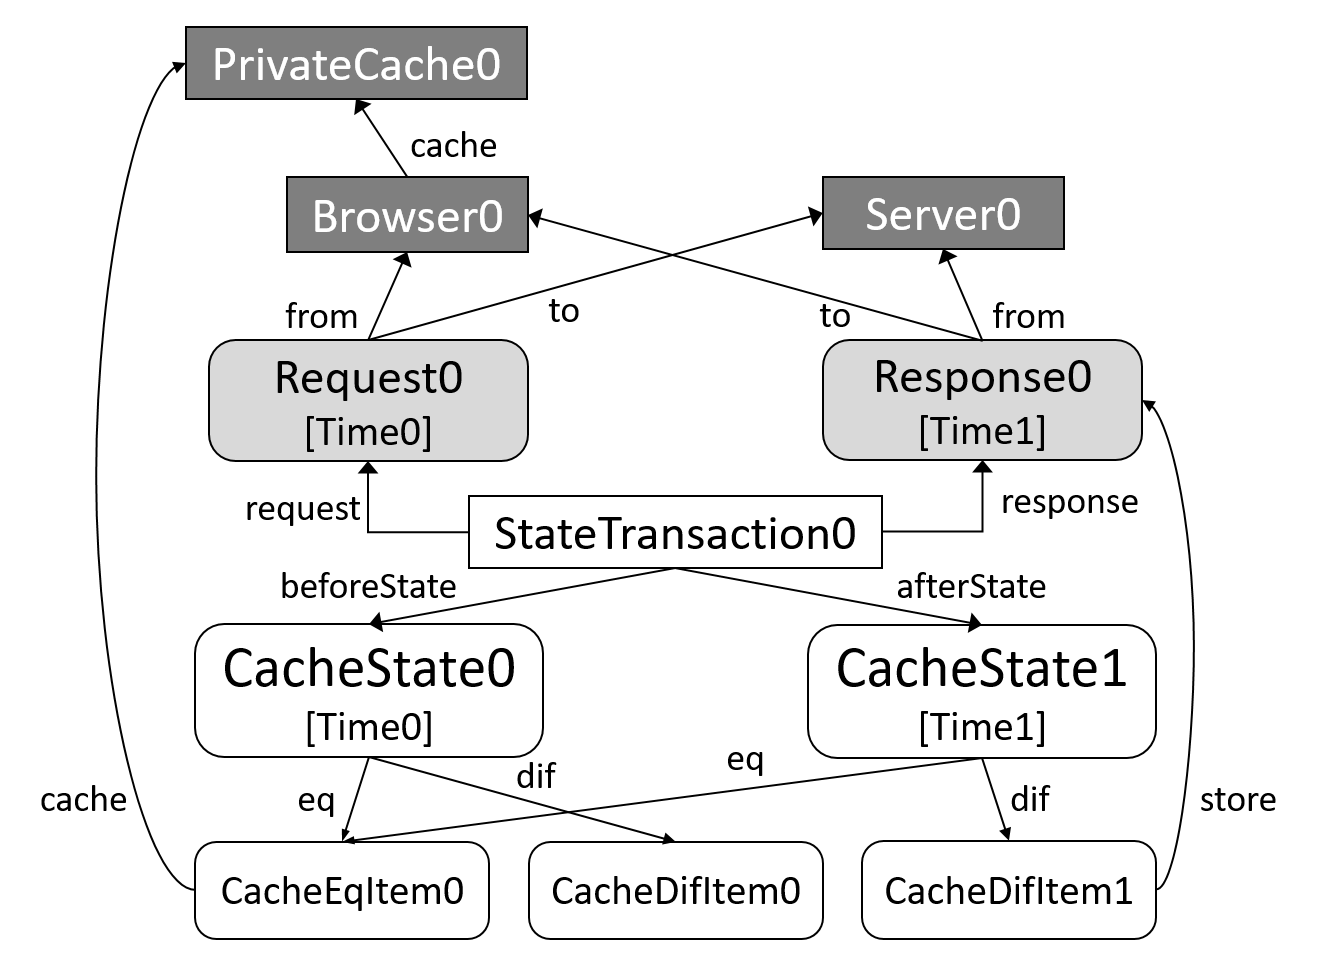
\includegraphics[width=450pt]{./fig/TestStore.eps}
\caption{レスポンスを格納する状態の一例}
\label{fig:TestStore}
\end{figure}

\subsection{格納レスポンスの再利用}
レスポンスの再利用動作を確認するため、実行結果からレスポンスの再利用を伴う動作を含む結果を抽出する。
ここでは簡単のため、最も単純な二者間における通信で生じるレスポンスの再利用を対象とし、Code\ref{code:test_reuse}を用いて出力を得る。
Code\ref{code:test_reuse}はクライアントとサーバの二者間における二組の通信において、一度レスポンスの再利用が発生している結果を出力するものである。

\begin{lstlisting}[caption=格納レスポンスの再利用, label=code:test_reuse]
run test_reuse{
	#HTTPClient = 1
	#HTTPServer = 1
	#Cache = 1

	#HTTPRequest = 2
	#HTTPResponse = 1
	#CacheReuse = 1
} for 4
\end{lstlisting}

得られる出力結果をスペースの都合上一部簡略化し、図\ref{fig:TestReuse}に示す。
図\ref{fig:TestReuse}はあるキャッシュを持つブラウザとサーバ間で、同様のURIに対してリクエストが二回送信された状態を表している。
ここで、StateTransaction0では図\ref{fig:TestStore}と同様、ブラウザキャッシュにResponse0を格納している。
StateTransaction1では、この格納レスポンスを再利用するイベントCacheReuse0が発生している。
以上より、図\ref{fig:TestReuse}に示す出力結果から、再利用を伴う動作が表現可能であることが確認できる。

\begin{figure}[htb]
\centering
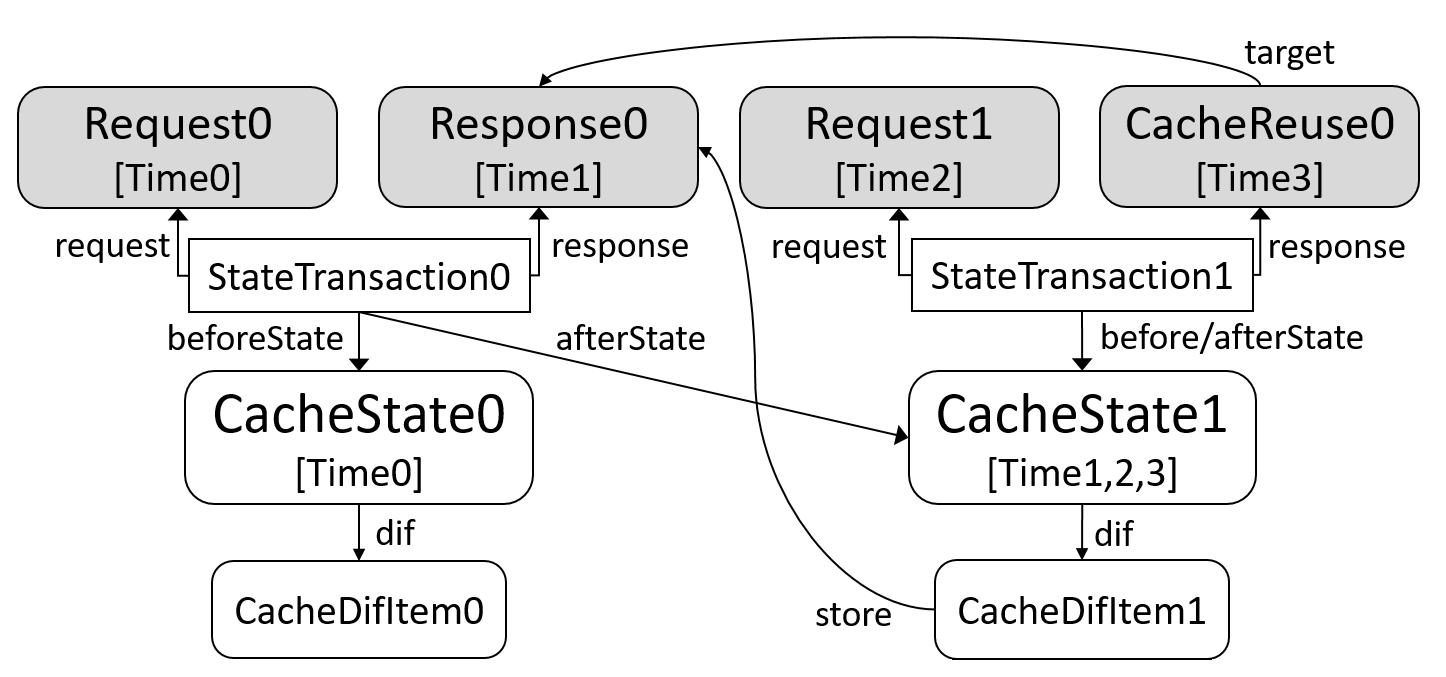
\includegraphics[width=450pt]{./fig/TestReuse.eps}
\caption{格納レスポンスを再利用する状態の一例}
\label{fig:TestReuse}
\end{figure}

\subsection{格納レスポンスの検証}
レスポンスの検証動作を確認するため、実行結果からレスポンスの検証を伴う動作を含む結果を抽出する。
ここでは簡単のため、最も単純な二者間における通信で生じるレスポンスの検証を対象とし、Code\ref{code:test_verification}を用いて出力を得る。
Code\ref{code:test_verification}はクライアントとサーバの二者間における三組の通信のうち、検証が行われた通信が存在する結果を出力する。
ここで検証が行われたかの判定は、\ref{sec:CacheVerification}節で述べたCode\ref{code:checkVerification}を利用している。

\begin{lstlisting}[caption=格納レスポンスの検証, label=code:test_verification]
run test_verification{
	#HTTPClient = 1
	#HTTPServer = 1
	#HTTPIntermediary = 0
	#Cache = 1
	#PrivateCache = 1

	some str:StateTransaction | checkVerification[str]
} for 6
\end{lstlisting}

得られる出力結果をスペースの都合上一部簡略化し、図\ref{fig:TestVerification}に示す。
図\ref{fig:TestVerification}はあるキャッシュを持つブラウザとサーバ間での、三つの通信(StateTransaction0,1,2)が存在している状態を表しており、このうちStateTransaction2が検証を行っている通信である。
まず、StateTransaction0では図\ref{fig:TestStore}と同様、ブラウザキャッシュにResponse0を格納している。
次に、Request2に対してブラウザキャッシュ内に格納されているResponse0を再利用するため、StateTransaction2で検証動作を行っている。
ここで、格納レスポンスのResponse0にはEtagHeaderが含まれているため、検証に用いる条件付きリクエストであるRequest1にはIfNoneMatchHeaderが含まれている。
また、検証結果となるResponse1は再利用可能であることを示す304の状態コードとなっているため、Response0はそのまま再利用可能であることが示されている。
以上を踏まえて、StateTransaction1ではResponse0をそのまま再利用している。

\begin{figure}[htb]
\centering
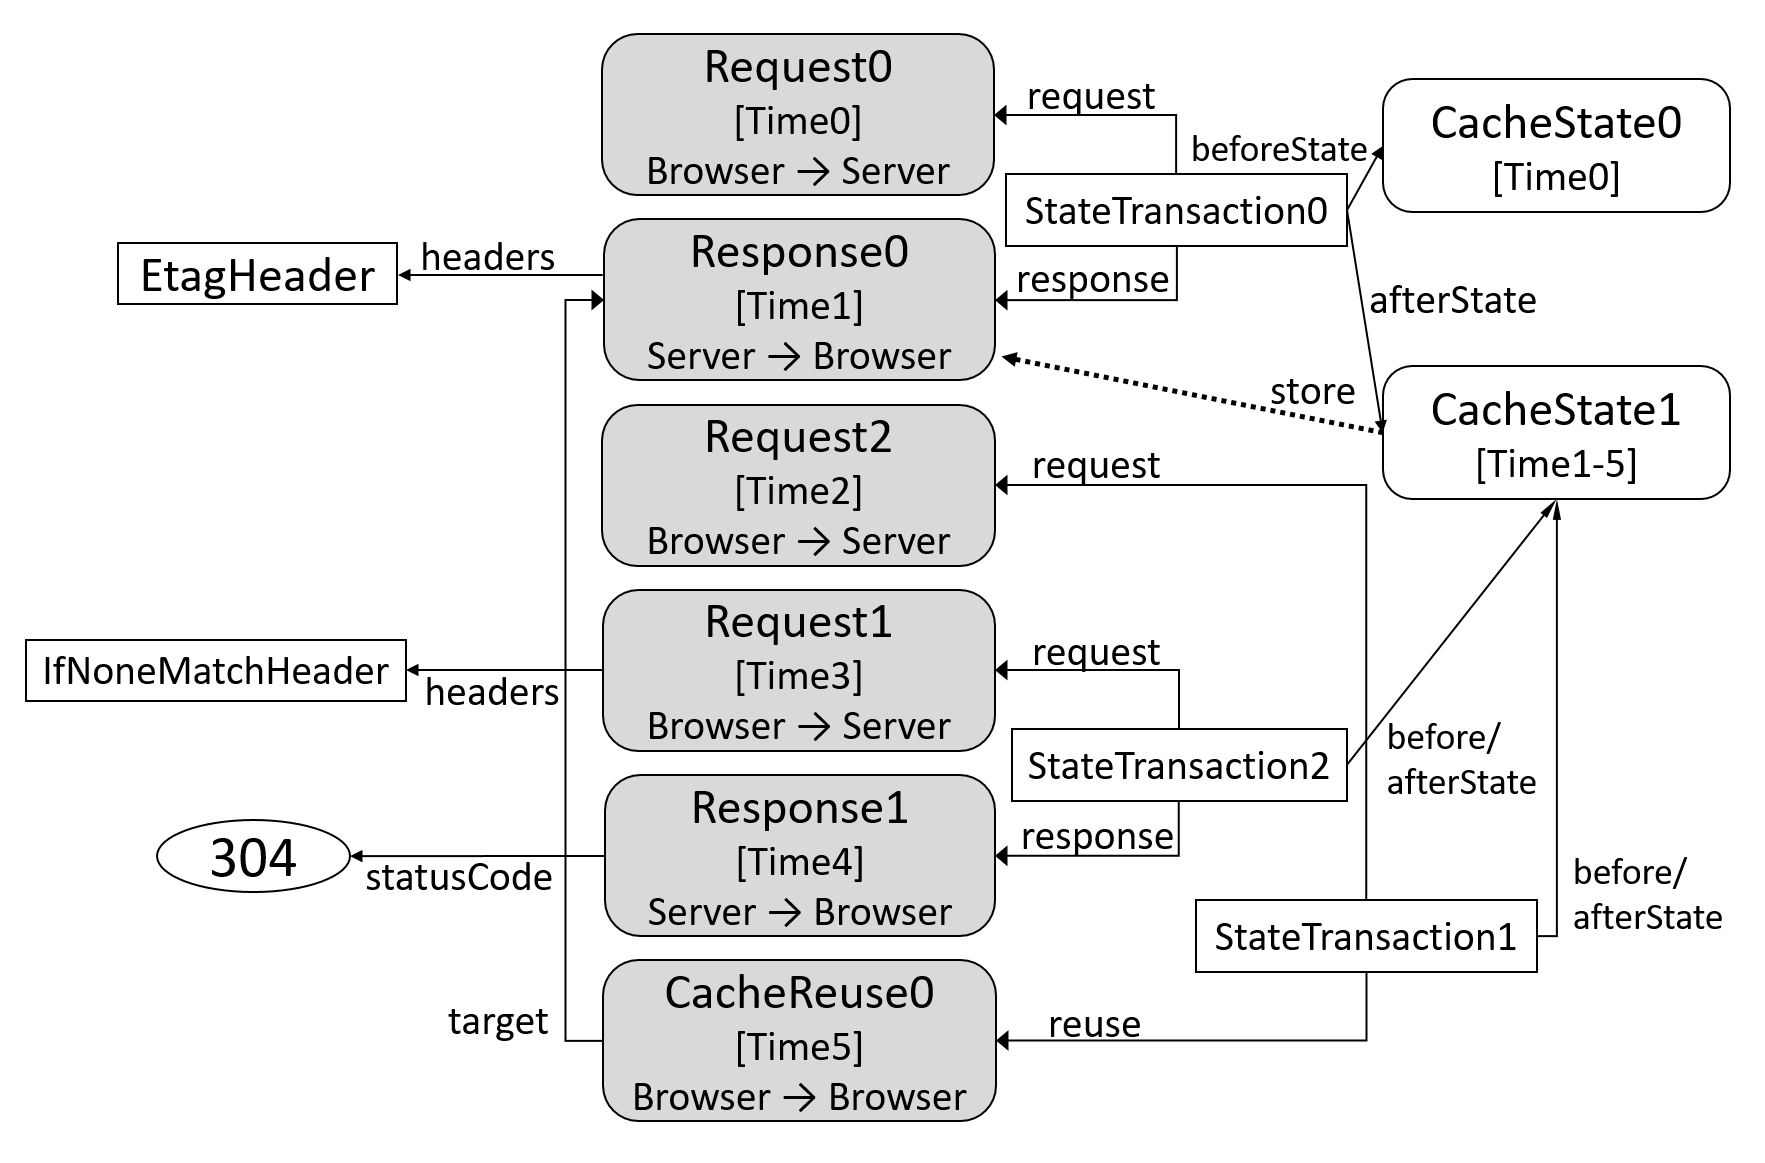
\includegraphics[width=450pt]{./fig/TestVerification.eps}
\caption{格納レスポンスの検証が含まれる状態の一例}
\label{fig:TestVerification}
\end{figure}

\section{中継者の基本動作}
中継者の動作を確認するため、実行結果から中継者の動作を伴う動作を含む結果を抽出する。
ここでは簡単のため、最も単純なクライアント、中継者、サーバが各一つずつ存在する経路において、中継者を経由する通信を対象としCode\ref{code:test_reuse}を用いて出力を得る。

\begin{lstlisting}[caption=中継者の動作, label=code:test_intermediary]
run test_intermediary{
	#HTTPRequest = 2
	#HTTPResponse = 2

	#HTTPClient = 1
	#HTTPServer = 1
	#HTTPIntermediary = 1

	all i:HTTPIntermediary | i in Alice.servers

	one req:HTTPRequest | req.to in HTTPIntermediary
	one req:HTTPRequest | req.to in HTTPServer
} for 4
\end{lstlisting}

得られる出力結果をスペースの都合上一部簡略化し、図\ref{fig:TestIntermediary}に示す。
図\ref{fig:TestIntermediary}で、HTTPTransaction0はブラウザと中継者間の通信、HTTPTransaction1は中継者とサーバ間の通信を表す。
中継者は自身に届けられたリクエストやレスポンスを回送する役割を持ち、このHTTPTransaction0,1が中継者による回送を表している。
以上より、中継者の動作が表現可能であることが確認できる。

\begin{figure}[htb]
\centering
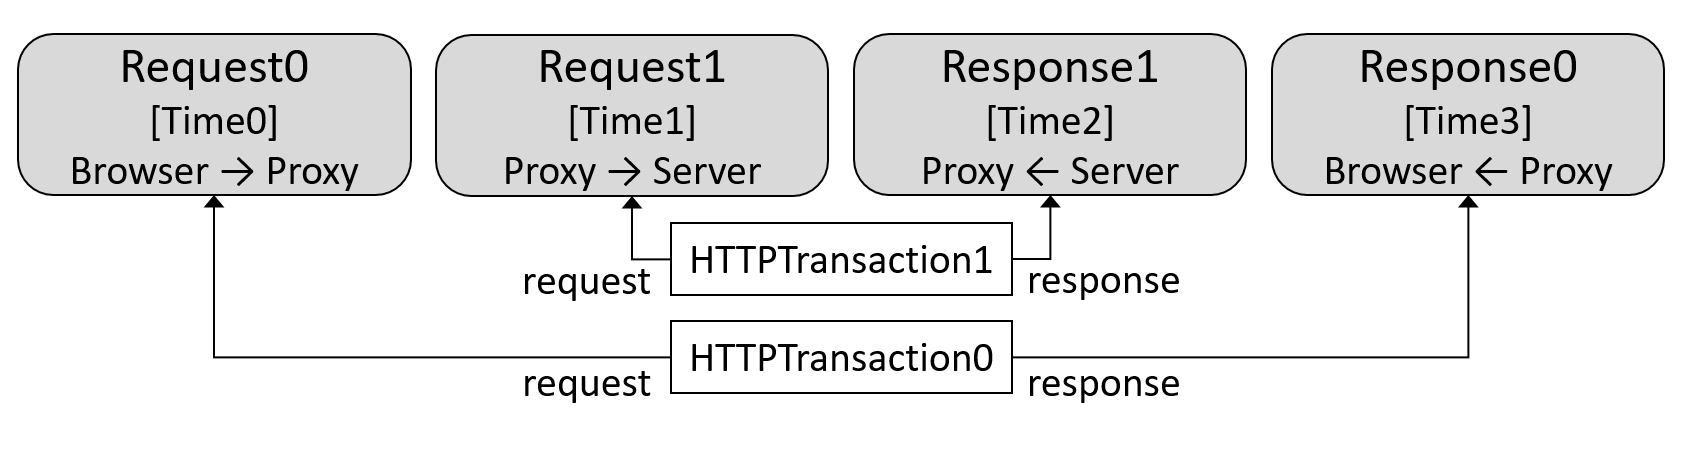
\includegraphics[width=450pt]{./fig/TestIntermediary.eps}
\caption{中継者の動作を含む状態の一例}
\label{fig:TestIntermediary}
\end{figure}

\section{Same-origin Browser Cache Poisoning Attack}
\label{sec:same-origin-bcp}
本節では、提案モデルでSame-origin Browser Cache Poisoning Attack\cite{bcpattack}(以下、Same-origin BCP攻撃とする)が表現可能であるかを確認する。

\subsection{攻撃の概要とフロー}
Same-origin BCP攻撃は、攻撃者の持つ中継者が攻撃対象であるブラウザとサーバの経路上に入り込む「中間者攻撃」の一種である。
本攻撃の目的は対象のブラウザ、攻撃者の任意の動作を実行させることを目的とする。
また、本攻撃の特徴は、攻撃者による通信経路の割り込みが一度であるにも関わらず、そのレスポンスを再利用するたびにブラウザが悪影響を受けるという影響の持続性にある。

攻撃全体のフローを図\ref{fig:SameBCP_flow}に示す。
本攻撃による攻撃者のふるまいは、通信経路上において本来ブラウザが受け取るはずのレスポンスの内容に改ざん(図\ref{fig:SameBCP_flow}内の「4.改ざんレスポンス」)を行い、ブラウザが保有するキャッシュに改ざんレスポンスを格納させることである。
この際の攻撃者による改ざん内容は以下の二点である。
\begin{itemize}
\item レスポンスのヘッダをブラウザキャッシュによるレスポンスの格納や再利用を誘発するよう改ざんする。例えば、有効期限の延長や、検証動作なしの再利用の許可が挙げられる
\item レスポンスのボディに攻撃者に実行させたい任意の動作を記述する
\end{itemize}
また、ブラウザに悪影響が及ぶのは「5.改ざんレスポンスをキャッシュに格納」時と「6.同じファイルの利用時に改ざんレスポンスを再利用」時である。
また、6は改ざんレスポンスがキャッシュ内に格納されている間、何度も繰り返される可能性がある。

\begin{figure}[htb]
\centering
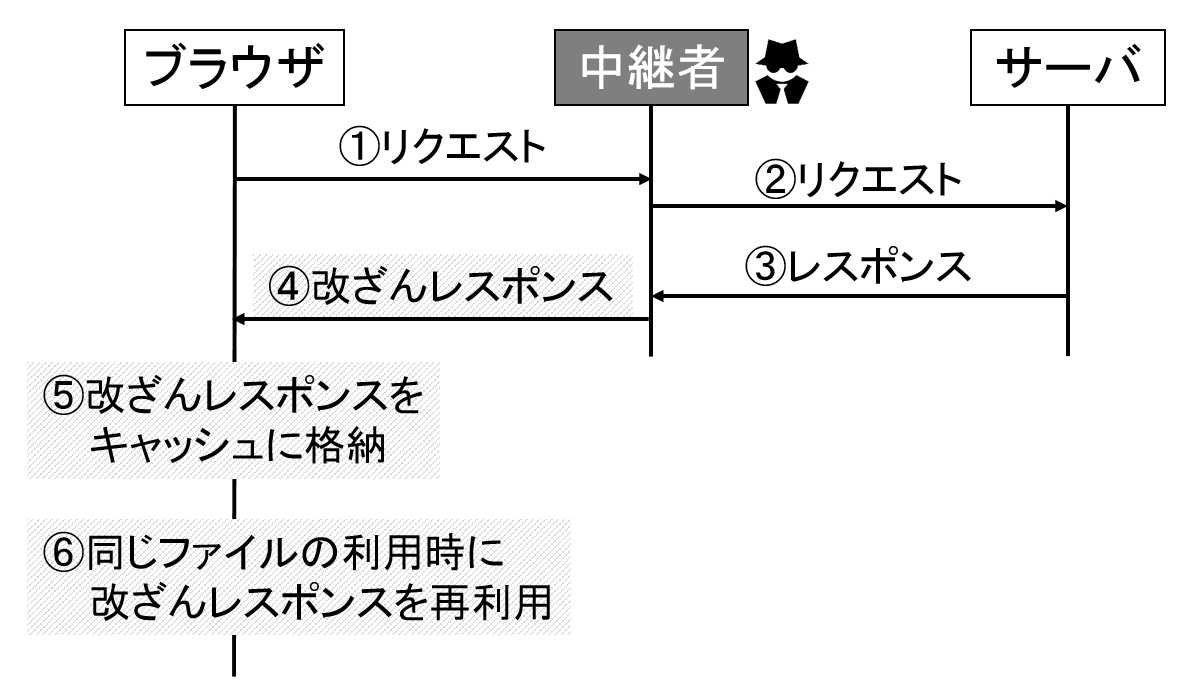
\includegraphics[width=400pt]{./fig/SameBCP_flow.eps}
\caption{Same-origin Browser Cache Poisoning Attackの攻撃フロー}
\label{fig:SameBCP_flow}
\end{figure}

\subsection{提案モデルによる出力}
提案モデルによるSame-origin BCP攻撃の表現を確認するため、実行結果から図\ref{fig:SameBCP_flow}のフローを含む結果を抽出する。
抽出にはCode\ref{code:Same_origin_BCP}を用いる。
実行結果として、図\ref{fig:SameBCP_flow}に従ったフローと、攻撃者によるヘッダとボディの改ざんを含む状態が得られた。
このことから、提案モデルがSame-origin BCP攻撃を表現できることを確認した。

\begin{lstlisting}[caption=Same-origin BCP攻撃の表現, label=code:Same_origin_BCP]
run Same_origin_BCP{
	#HTTPClient = 1
	#HTTPServer = 1
	#HTTPIntermediary = 1
	#PrivateCache = 1
	#PublicCache = 0

	#HTTPRequest = 3
	#HTTPResponse = 2
	#CacheReuse = 1

	#Principal = 3
	#Alice = 2

	some tr,tr',tr'':HTTPTransaction | {
		tr'.request.current in tr.request.current.*next
		tr.response.current in tr'.response.current.*next
		tr''.request.current in tr.response.current.*next
		some tr''.re_res

		tr.request.from in HTTPClient
		tr.request.to in HTTPIntermediary

		tr'.request.from in HTTPIntermediary
		tr'.request.to in HTTPServer

		tr''.request.from in HTTPClient

		tr.response.body != tr'.response.body
	}

	some c:HTTPClient | c in Alice.httpClients
	some s:HTTPServer | s in Alice.servers
	no i:HTTPIntermediary | i in Alice.servers
} for 6
\end{lstlisting}

\section{Cross-site Request Forgeries Attack}
本節では、提案モデルでCross-site Request Forgeries Attack\cite{cookie-model}(以下、CSRF攻撃とする)が表現可能であるかを確認する。

\subsection{攻撃の概要とフロー}
CSRF攻撃は攻撃対象となるサーバと攻撃者が保有するサーバ、そして一般的なブラウザの三者間で実現される攻撃である。
本攻撃の目標は、攻撃対象であるサーバに対して、攻撃者が許されていない動作を実行させることである。

攻撃全体のフローを図\ref{fig:CSRF_flow}に示す。
本攻撃における攻撃者のふるまいは、自身が保有するサーバにアクセスしてきたブラウザが攻撃対象であるサーバへのリクエスト(図\ref{fig:SameBCP_flow}内の「3.リクエスト」)を送信を誘発するようにレスポンス(図\ref{fig:SameBCP_flow}内の「2.レスポンス」)を返すことである。
また、この攻撃者からのレスポンスの内容によって、ブラウザから送信されるリクエストも操作される。

\begin{figure}[htb]
\centering
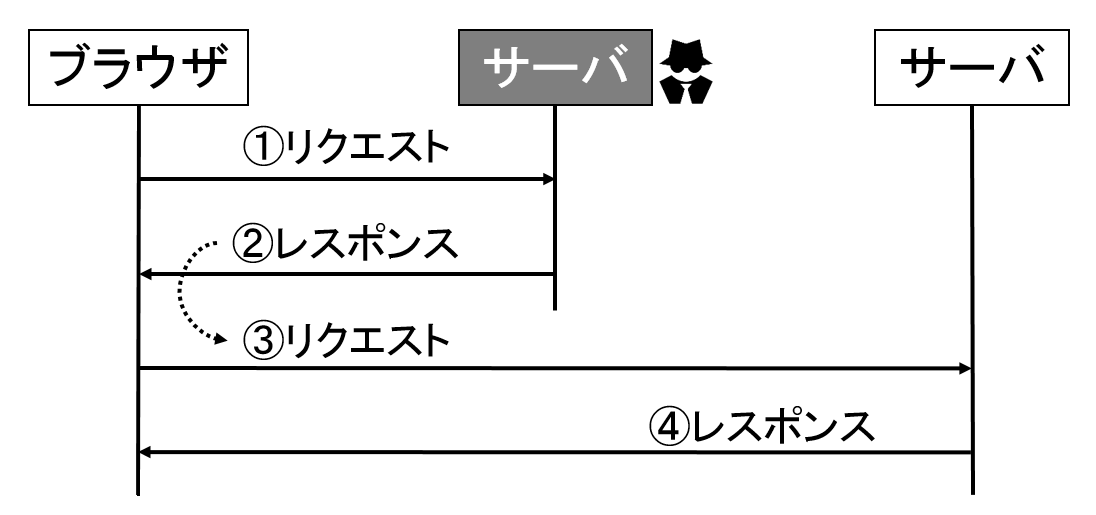
\includegraphics[width=400pt]{./fig/CSRF_flow.eps}
\caption{Cross-site Request Forgeries Attackの攻撃フロー}
\label{fig:CSRF_flow}
\end{figure}

\subsection{提案モデルによる出力}
提案モデルによるCSRF攻撃の表現を確認するため、実行結果から図\ref{fig:CSRF_flow}のフローを含む結果を抽出する。
抽出にはCode\ref{code:CSRF}を用い、その実行結果として図\ref{fig:CSRF_flow}に示す攻撃フローを含む結果が出力された。
スペースの都合上、これを一部簡略化し図\ref{fig:CSRF_alloy}に示す。
図\ref{fig:CSRF_alloy}において、Server0が攻撃者のサーバ、Server1が攻撃対象のサーバを表している。
また、HTTPTransaction0はBrowserがServer0にアクセスした通信を、HTTPTransaction1はそれに誘発されたBrowserとServer1の通信を表している。
HTTPTransaction1はHTTPTransaction0にcauseの関係を持ち、これがHTTPTransaction0に誘発されていることを示している。
以上のことから、CSRF攻撃を含む出力結果が得られているため、提案モデルがCSRF攻撃を表現できることを確認した。

\begin{lstlisting}[caption=CSRF攻撃の表現, label=code:CSRF]
run CSRF{
	#HTTPRequest = 2
	#HTTPResponse = 2

	#HTTPClient = 1
	#HTTPServer = 2
	#HTTPIntermediary = 0

	#Principal = 3
	#Alice = 2

	all p:Principal |
		one c:HTTPConformist |
			c in p.(servers + httpClients)
	all b:Browser | b in Alice.httpClients

	one tr1,tr2:HTTPTransaction|{
		tr2.request.current in tr1.response.current.*next

		tr1.request.to !in Alice.servers
		tr2.request.to in Alice.servers

		tr2.cause = tr1

		tr1.request.uri != tr2.request.uri
	}
} for 4
\end{lstlisting}

\begin{figure}[htb]
\centering
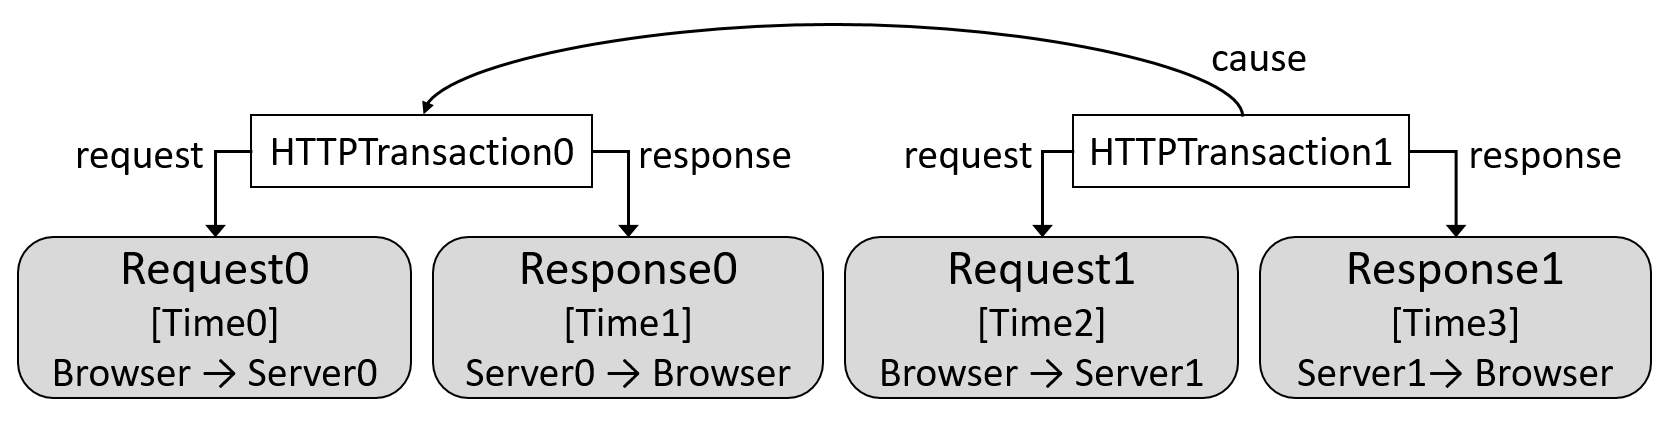
\includegraphics[width=450pt]{./fig/CSRF_alloy.eps}
\caption{CSRF攻撃のフローを含む状態の一例}
\label{fig:CSRF_alloy}
\end{figure}

\section{Cross-origin Browser Cache Poisoning Attack}
本節では、提案モデルでCross-origin Browser Cache Poisoning Attack\cite{bcpattack}(以下、Cross-origin BCP攻撃とする)が表現可能であるかを確認する。

\subsection{攻撃の概要とフロー}
Cross-origin BCP攻撃は、\ref{sec:same-origin-bcp}節で述べたSame-origin BCP攻撃と同様に「中間者攻撃」一種である。
Same-origin BCP攻撃に比べ、改ざんレスポンスの再利用の頻度を高めることができる。
これは、Cross-origin BCP攻撃では、任意のファイルのレスポンスに改ざんを行うことができることに起因する。
これにより、一つのサイトだけでなく多くのサイトに共通して利用されるようなファイル(cssやjsファイルなど)を改ざんの対象とすることができる。
これに対して、\ref{sec:same-origin-bcp}節で記述のSame-origin BCP攻撃は、攻撃者がファイルを指定することはできず、通信に介入した際に偶然行われていた通信のみを改ざん可能な対象とする。

Cross-origin BCP攻撃は図\ref{fig:CrossBCP_flow}に示す攻撃フローで実現される。
ここで、図\ref{fig:CrossBCP_flow}内での「5.リクエスト」以降は、Same-origin BCP攻撃と同一のフローである。
また、それ以前のフローについては、CSRFのフローと役割が類似している。
まず最初に、攻撃者は「1.リクエスト」の通信に介入し、レスポンスの改ざんを行う。
ここにおける改ざんは、実際に改ざんを試みるファイルに対しての「5.リクエスト」の誘発を目的とする。
例えば、「A.css」という多くのページで共通して使用されるファイルが存在する場合、「3.レスポンス」の内容にA.cssを利用するよう追記することで、A.cssに対する「5.リクエスト」を誘発することができる。
したがって、図\ref{fig:CrossBCP_flow}のフローによって、攻撃者が指定する任意のファイルの改ざんを行い、そのレスポンスをブラウザキャッシュに格納させることができる。
また、このフローの成功後はサーバ1,2に無関係な通信であったとしても、改ざんレスポンスに記述されているファイルを利用する際には再利用が発生し、ブラウザは悪影響を受ける。

\begin{figure}[htb]
\centering
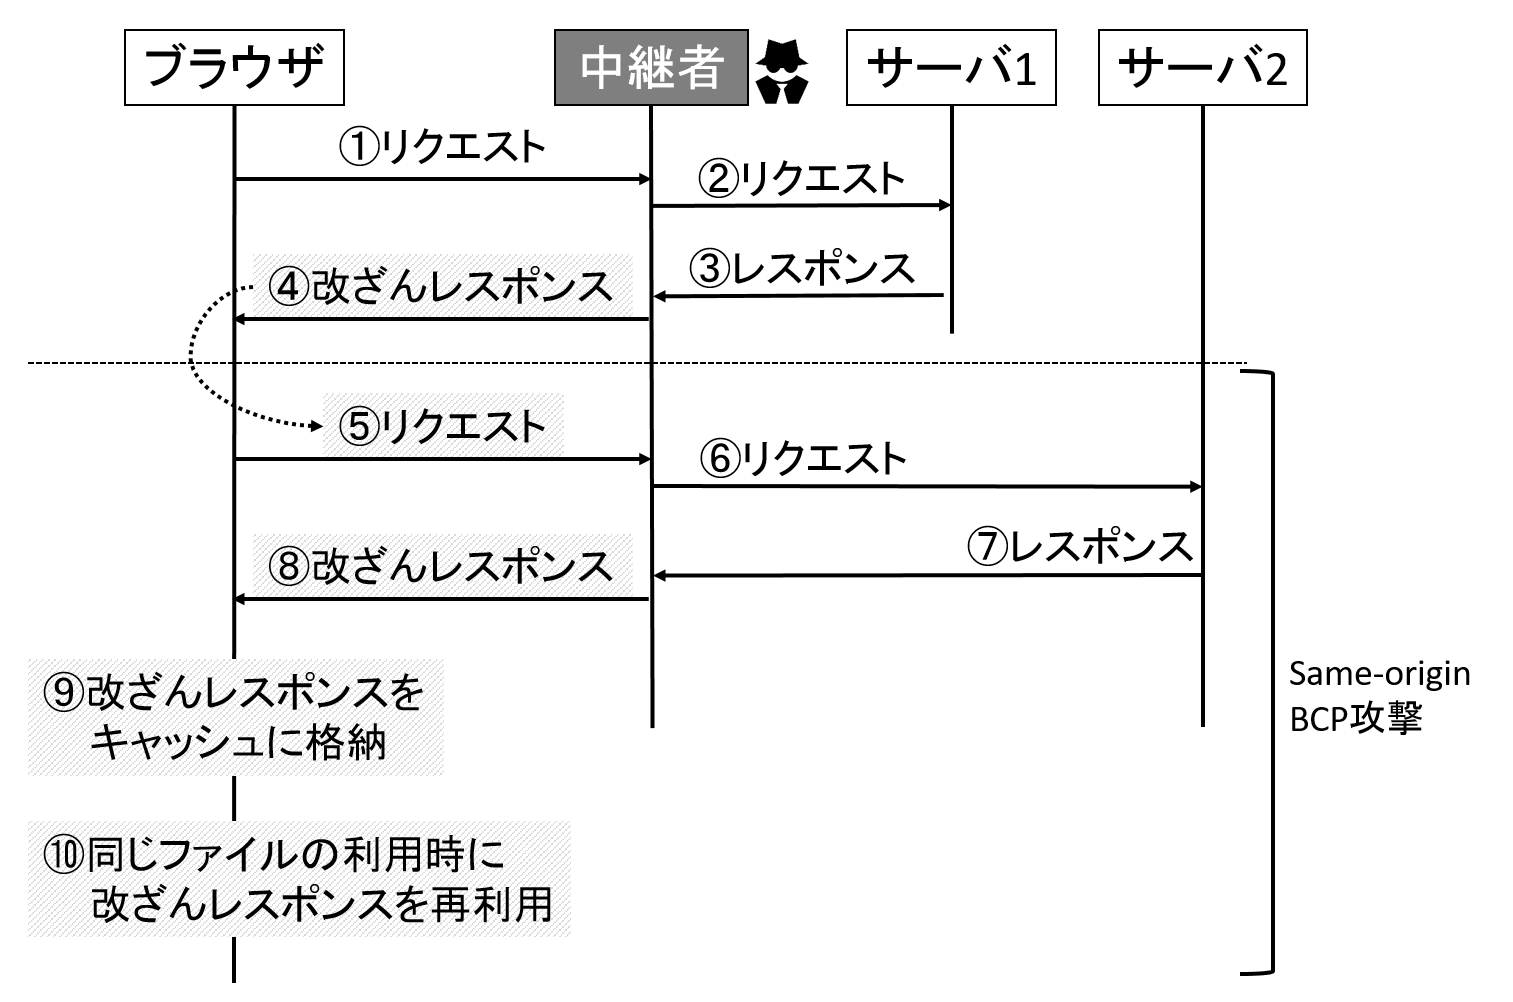
\includegraphics[width=450pt]{./fig/CrossBCP_flow.eps}
\caption{Cross-origin Browser Cache Poisoning Attackの攻撃フロー}
\label{fig:CrossBCP_flow}
\end{figure}

\subsection{提案モデルによる出力}
提案モデルによるCSRF攻撃の表現を確認するため、実行結果から図\ref{fig:CrossBCP_flow}を含む結果を抽出する。
結果として、図\ref{fig:CrossBCP_flow}に存在する五つの通信を表現された状態を出力した。
このことから、提案モデルがCross-origin BCP攻撃を表現できることを確認した。
また、スペースの都合上、実行コードは巻末付録Code\ref{code:Cross_origin_BCP}に記載する。

\section{Web Cache Deception Attack}
本節では、提案モデルでWeb Cache Deception Attack\cite{WCD}(以下、WCD攻撃とする)が表現可能であるかを確認する。

\subsection{攻撃の概要とフロー}
WCD攻撃は攻撃対象となるサーバと中継者、二つのブラウザで成り立つ攻撃である。
攻撃者はこれらのうち一つのブラウザを所有し、本来、攻撃者がサーバから得ることのできないファイルを取得することが目的である。

WCD攻撃は図\ref{fig:WCD_flow}に示す攻撃フローで実現される。
まず、攻撃者にアクセス権の無いファイルに対して、正当なユーザに中継者を経由してアクセスさせる。
この際に、そのレスポンス(図\ref{fig:WCD_flow}内の「3.レスポンス」)が中継者のキャッシュに格納された場合、攻撃者はその中継者を含む経路でそのファイルに対するリクエスト(図\ref{fig:WCD_flow}内の「5.リクエスト」)を送信することで、そのファイルを取得することができる(図\ref{fig:WCD_flow}内の「6.格納レスポンスの再利用」)。

\begin{figure}[htb]
\centering
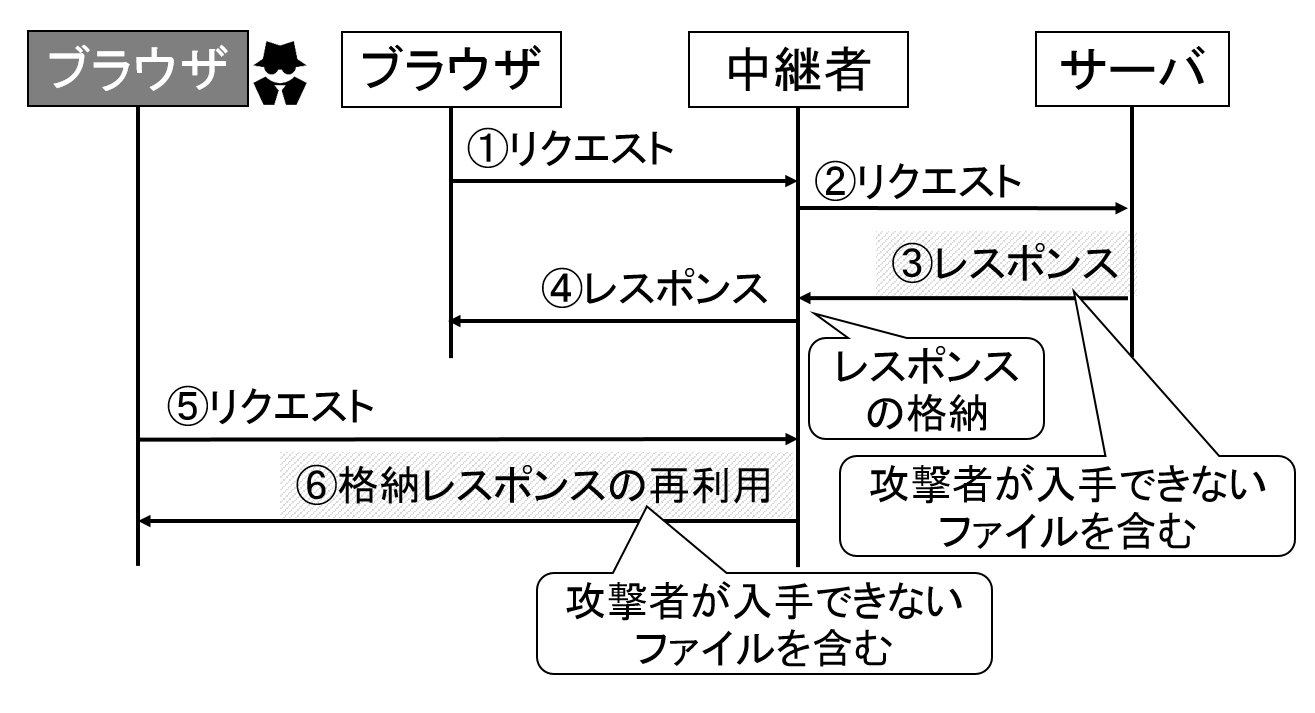
\includegraphics[width=450pt]{./fig/WCD_flow.eps}
\caption{Web Cache Deception Attackの攻撃フロー}
\label{fig:WCD_flow}
\end{figure}

\subsection{提案モデルによる出力}
提案モデルによるWCD攻撃の表現を確認するため、実行結果から図\ref{fig:WCD_flow}のフローを含む結果を抽出する。
抽出にはCode\ref{code:WCD}を用い、その実行結果として図\ref{fig:WCD_flow}に示す攻撃フローを含む結果が出力された。
スペースの都合上、これを一部簡略化し図\ref{fig:WCD_alloy}に示す。
図\ref{fig:WCD_alloy}において、図\ref{fig:WCD_flow}の「1.リクエスト」と「2.リクエスト」の通信はStateTransaction0,1でそれぞれ表されている。
ここで、Response1のボディにはTokenが付与されており、これが攻撃者がアクセス権を持たないファイルを示している。
このResponse1は、その発生時刻Time2で中継者のキャッシュに保存され、攻撃者による通信StateTransaction2において再利用されている。
従って、この出力結果は攻撃者が本来権限を持たないファイルを中継者のキャッシュによる再利用を用いて取得していることを表している。
以上のことから、WCD攻撃を含む出力結果が得られているため、提案モデルがWCD攻撃を表現できることを確認した。

\begin{lstlisting}[caption=WCD攻撃の表現, label=code:WCD]
run Web_Cache_Deception{
	#HTTPRequest = 3
	#HTTPResponse = 2
	#CacheReuse = 1

	#HTTPClient = 2
	#HTTPServer = 1
	#HTTPProxy = 1
	#Cache = 1

	#Principal = 4
	#Alice = 3

	all c:Cache | c in HTTPProxy.cache

	all p:Principal |
		one c:HTTPConformist |
			c in p.(servers + httpClients)
	all i:HTTPProxy | i in Alice.servers
	all s:HTTPServer | s in Alice.servers

	one tr1,tr2,tr3:HTTPTransaction |{
		tr1.request.from in Alice.httpClients
		tr1.request.to in HTTPProxy

		tr2.request.from in HTTPProxy
		tr2.request.to in HTTPServer

		(tr3.request.from !in Alice.httpClients and tr3.request.from in HTTPClient)
		tr3.request.to in HTTPProxy

		one tr3.re_res
	}
} for 6
\end{lstlisting}

\begin{figure}[htb]
\centering
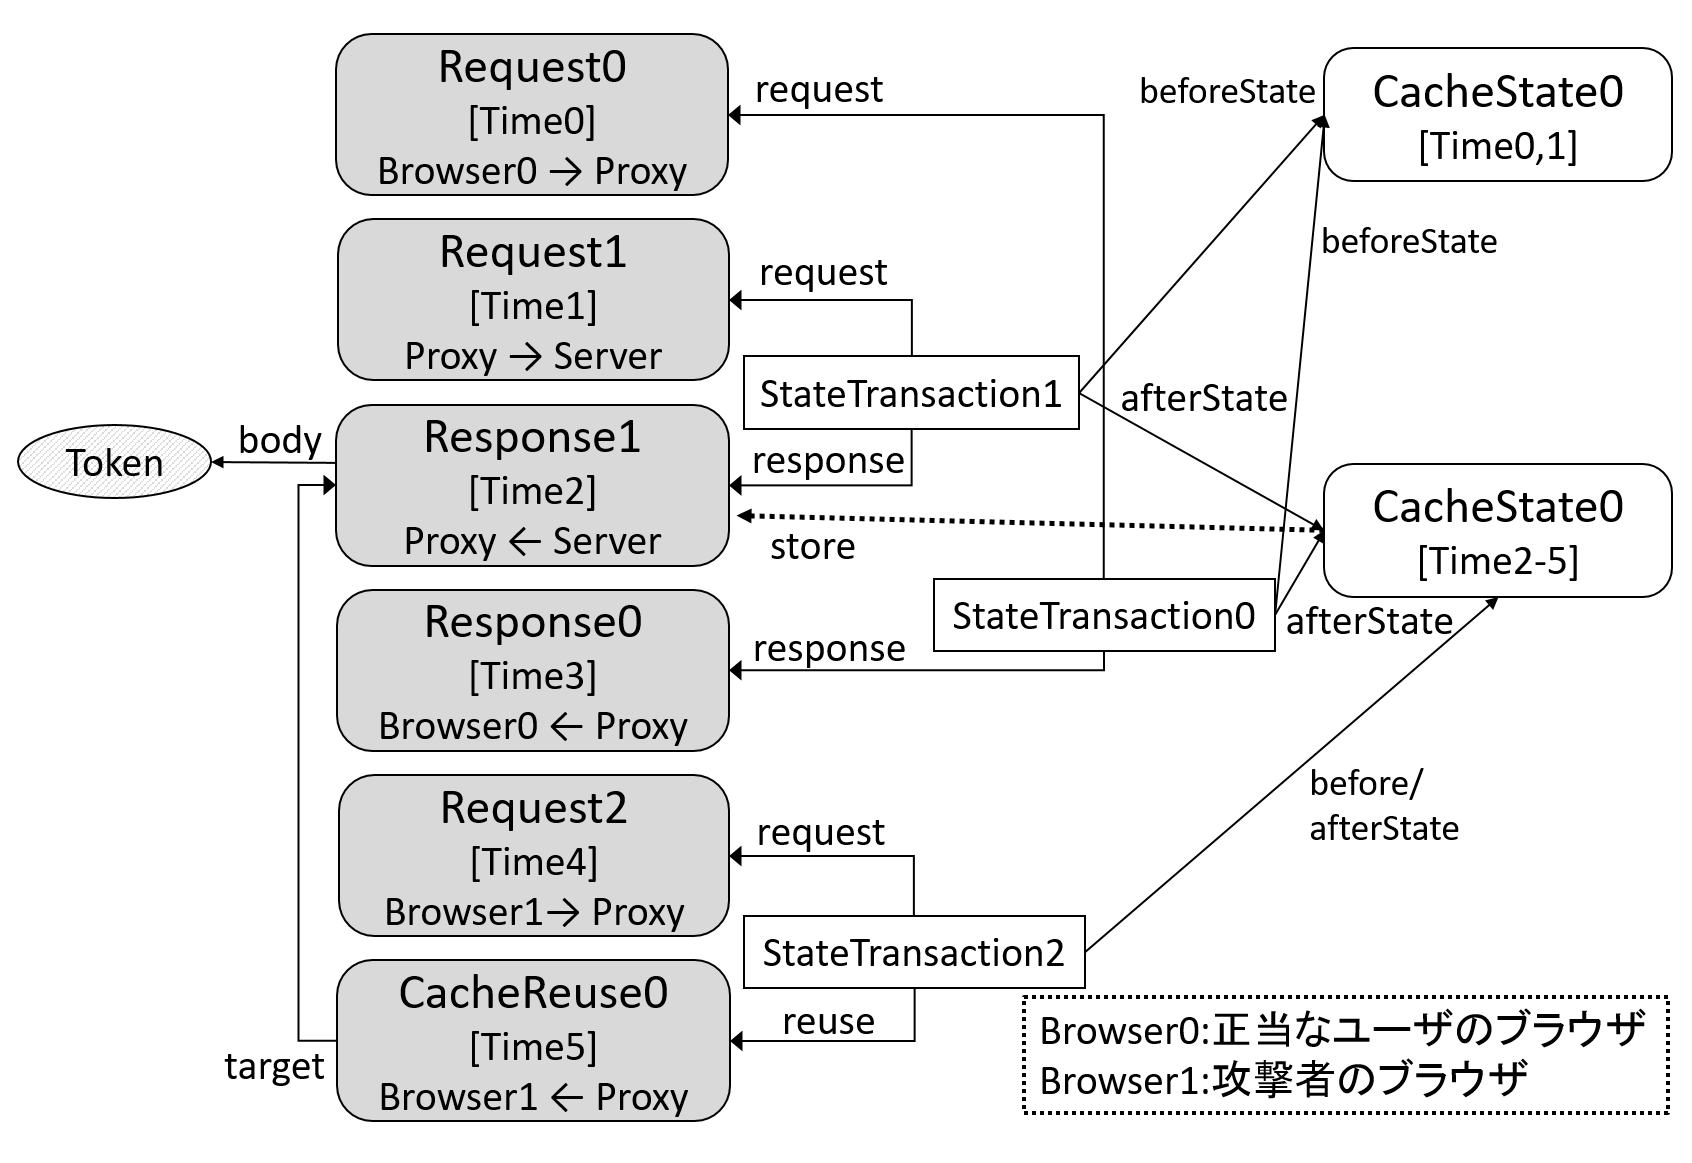
\includegraphics[width=450pt]{./fig/WCD_alloy.eps}
\caption{WCD攻撃のフローを含む状態の一例}
\label{fig:WCD_alloy}
\end{figure}

\end{document}
